\subsection{Оптимизация системы охлаждения ГТУ}
Одной из особенностей проектируемой ГТУ является предварительное захолаживание воздуха, охлаждающего турбину высокого давления, во внешнем воздухо-водяном теплообменном аппарате. Данная конструкция позволяет сильно уменьшить температуру охлаждающего воздуха (с 771 К - температура нв выходе из КВД до 500 К - температура на входе в ТВД). Кроме того, вывод охлаждающего воздуха за пределы корпуса позволяет также использовать дожимающий компрессор для увеличения давления воздуха, что позволит осущестлять его выдув в лобовой точке соплового аппарата турбины высокого давления.

Схема установки с дожимающим компрессором представлена на рис. ~\ref{img:sub_compress_scheme}.

\begin{figure}[H]
    \centering
    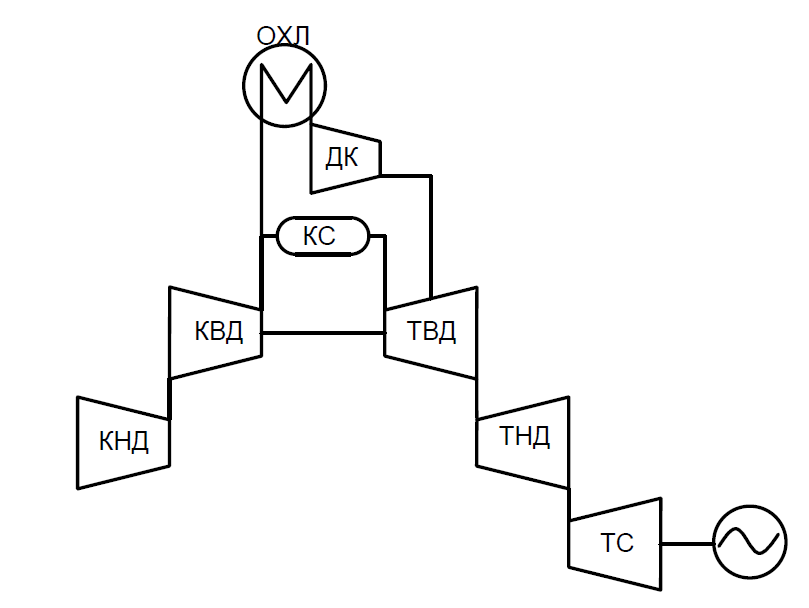
\includegraphics[scale=0.6]{sub_compress_scheme}
    \caption{Схема установки с дожимающим компрессором}
	\label{img:sub_compress_scheme}
\end{figure}

В данной работе был проведен анализ эффективности этого конструктивного решения, с точки зрения параметров установки на номинальном режиме, а также с точки зрения оптимизации системы охлаждения. 

Подробный расчет системы охлаждения соплового аппарата приведен ниже.

При оценке влияния дожимающего компрессор на цикл установки, его параметры принимались следующими: степень повышения давления $\pi_{д.к.} = 1,2$, а его КПД $\eta_{д.к.} = 0,85$.
Расход воздуха через дожимающий компрессор определялся из условия обеспечения наибольшей температуры металла соплового аппарата 1000 К (графики распределения температуры будут показаны ниже).

Без выдува в лобовую точку относительная доля охлаждающего воздуха, отводимого из компрессора высокого давления, составляет 10\%, что в абсолютном значении составляет 5,11 кг/c. Применение дожимающего компрессора позволило уменьшить эту величину до 9,64\%, что в абсолютном значении составляет 4,92\%. 

На рис. ~\ref{img:sub_compress_cycle} представлен график относительных параметров установки с дожиманием на номинальном режиме.  

\begin{figure}[H]
    \centering
    \includegraphics[scale=0.6]{img:sub_compress_cycle}
    \caption{Параметры установки с дожимающим компрессором на номинальном режиме}
	\label{img:sub_compress_cycle}
\end{figure}

В точке, соответствюущей максимальному КПД установка имеет параметры, представленные в таблице ~\ref{tab:cycle_sub_compress_max_eta}. При этом удельная работа дожимающего компрессора обозначена, как $L_{e \ д.к.}$, МДж/кг, а расхода - как $G_{д.к.}$, кг/с.
\begin{longtable}{|c|c|c|c|c|c|}
	\caption{Параметры двухвальной безрегенеративной установки в точке, соответствующей максимальному КПД} 
	\label{tab:cycle_sub_compress_max_eta}
	\hline
	\textbf{$\pi_к$} & \textbf{$\eta_e$} & \textbf{$L_e, \ МДж/кг$} & \textbf{$G_в, \ кг/с$} & \textbf{$L_{e \ д.к.}, \ МДж/кг$} & \textbf{$G_{д.к.}, \ кг/с$} \\ \hline
	16,5 & 0,270 & 0,325 & 59,2 \\ \hline
\end{longtable}

В точке, соответствующей максимальном КПД установка имеет параметры, представленные в таблице ~\ref{tab:cycle_sub_compress_max_labour}.
\begin{longtable}{|c|c|c|c|}
	\caption{Параметры двухвальной безрегенеративной установки в точке, соответствующей максимальному КПД} 
	\label{tab:cycle_sub_compress_max_labour}
	\hline
	\textbf{$\pi_к$} & \textbf{$\eta_e$} & \textbf{$L_e, \ МДж/кг$} & \textbf{$G_в, \ кг/с$} & \textbf{$L_{e \ д.к.}, \ МДж/кг$} & \textbf{$G_{д.к.}, \ кг/с$} \\ \hline
	16,5 & 0,270 & 0,325 & 59,2 \\ \hline
\end{longtable}

Как можно заметить, использование дожимающего компрессора приводит к небольшому снижению КПД установки, однако данное снижение представляется оправданным в связи с уменьшением температурной неравномерности в материале соплового аппарата турбины выского давления (показано ниже).